\chapter{ALGORITHM FOR GRAPHS}
\label{chap:graph}
 
In this chapter we discuss about our proposed algorithm for graphs. 
Given is a Graph $G \equiv (V,E)$ where $V$ is total number of vertices and $E$ is total number of edges.

The drawback of proposed algorithm of DAG was huge memory requirement so it is not feasible to apply the same algorithm for graphs. 
What we observed is that Brandes' algorithm makes each and every vertex as a source in any order and performs BFS. But we can select an order such that we can reuse partial BFS graph which are commmon for two vertices. Such an ordering is possible, if we compute BFS for vertex $v$ then for any neighbour $u$ of $v$ we can reuse that graph partially, provided that $u$ has not yet been considered for BFS. Similarly, $u$'s graph can be reused for all its neighbours if they are not considered for BFS.

For a source $w$, the graph which gets formed while BFS has its edges classified at every vertex as $parent$, $cousins$, $children$.
While performing BFS, if there is a vertex $v$ at height $h$ and another vertex $u$ at height $h+1$ and there is an edge between $v$ and $u$ then for vertex $v$, vertex $u$ is $child$ and for vertex $u$, vertex $v$ is $parent$.
If there is an edge in original graph between any two vertices and not included in BFS graph, then they are $cousins$ of each other.
For source $w$, its $parent$ and $cousins$ remains to be empty set.

In Figure \ref{fig:exgraph1} vertex 0 is considered as source and in Figure \ref{fig:exgraph2}, vertex 1 is considered as source. These graphs are BFS graph which consists of dotted edges representing $cousins$ and directed edges represent $parent$ to $child$ relation.

\begin{figure}
%\centering
\hspace{-4.5em}
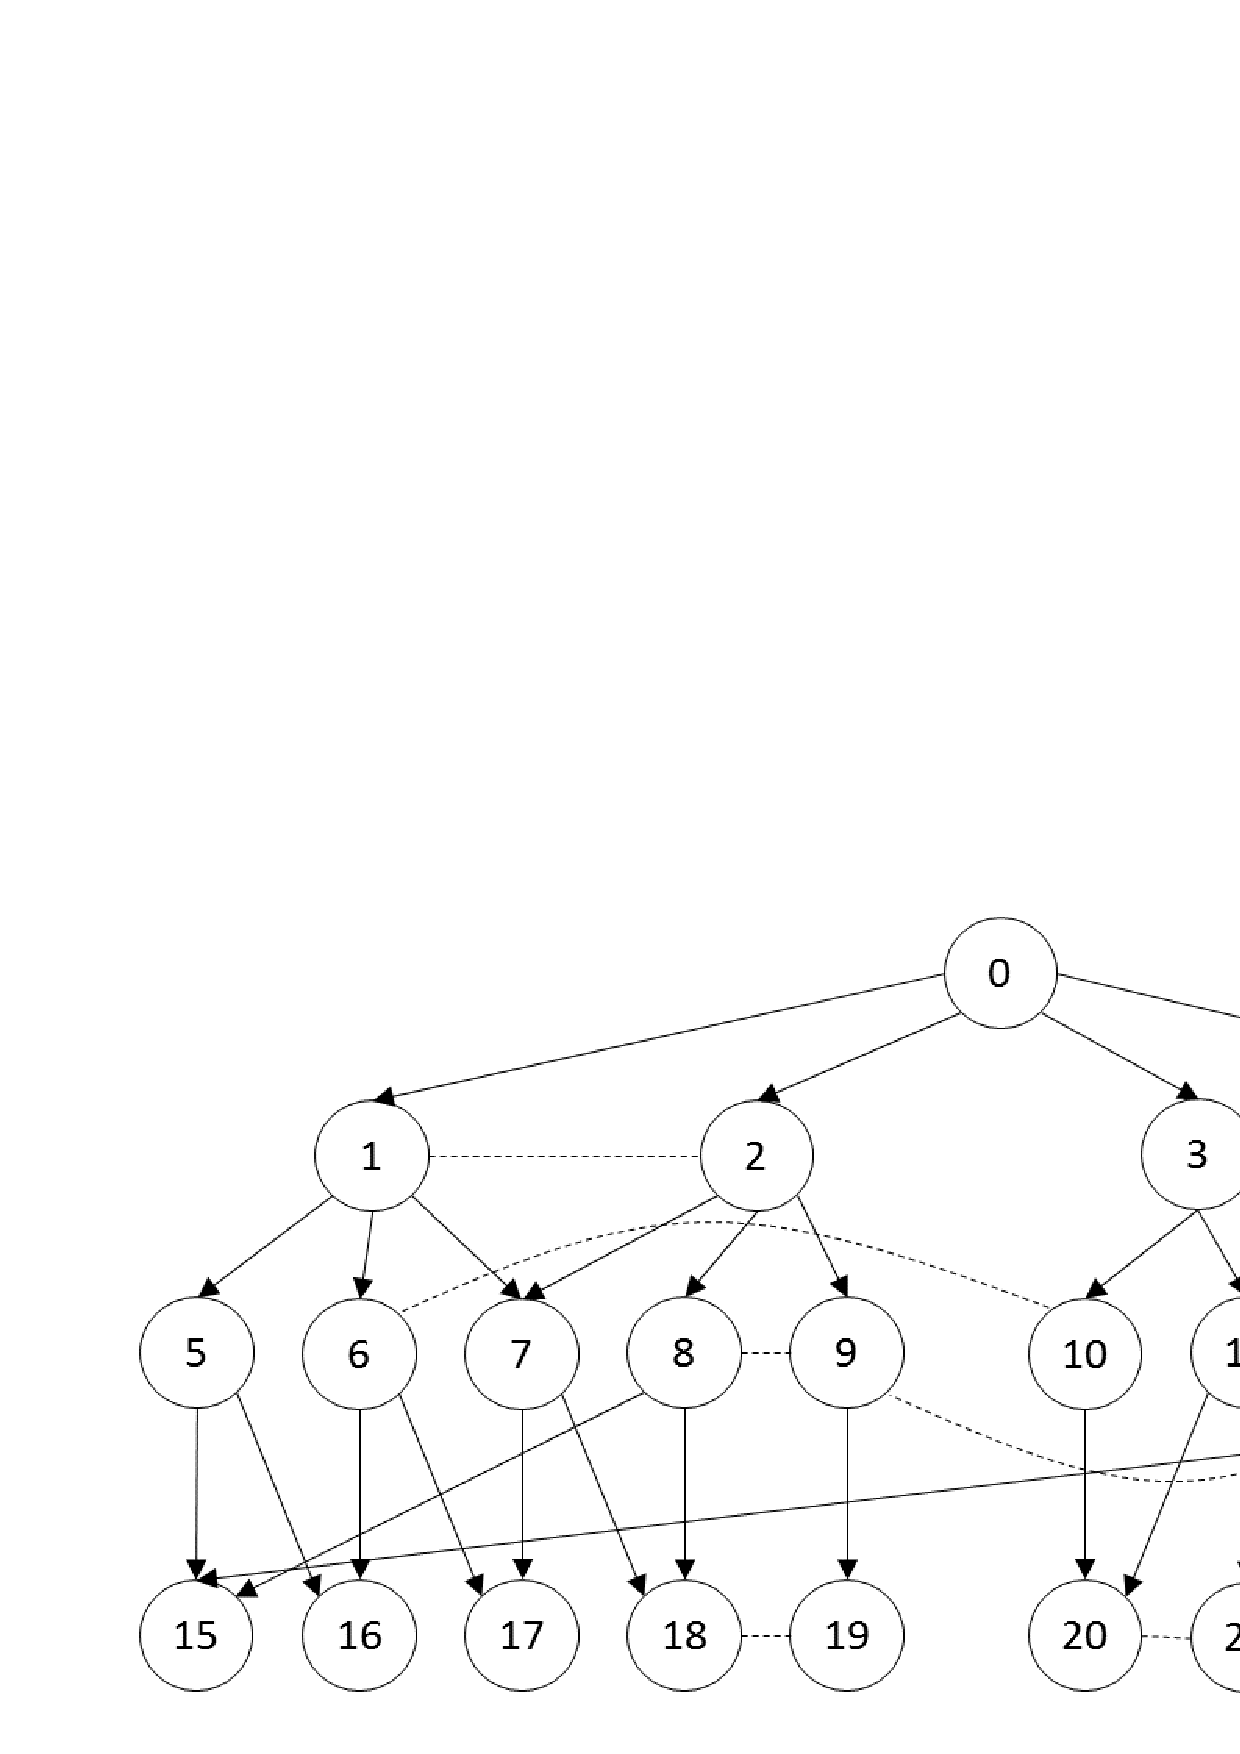
\includegraphics[width=19cm]{images/Slide1.PNG}
\caption{BFS with vertex 0 as source}
\label{fig:exgraph1}
\end{figure}

\begin{figure}
%\centering
\hspace{-4.5em}
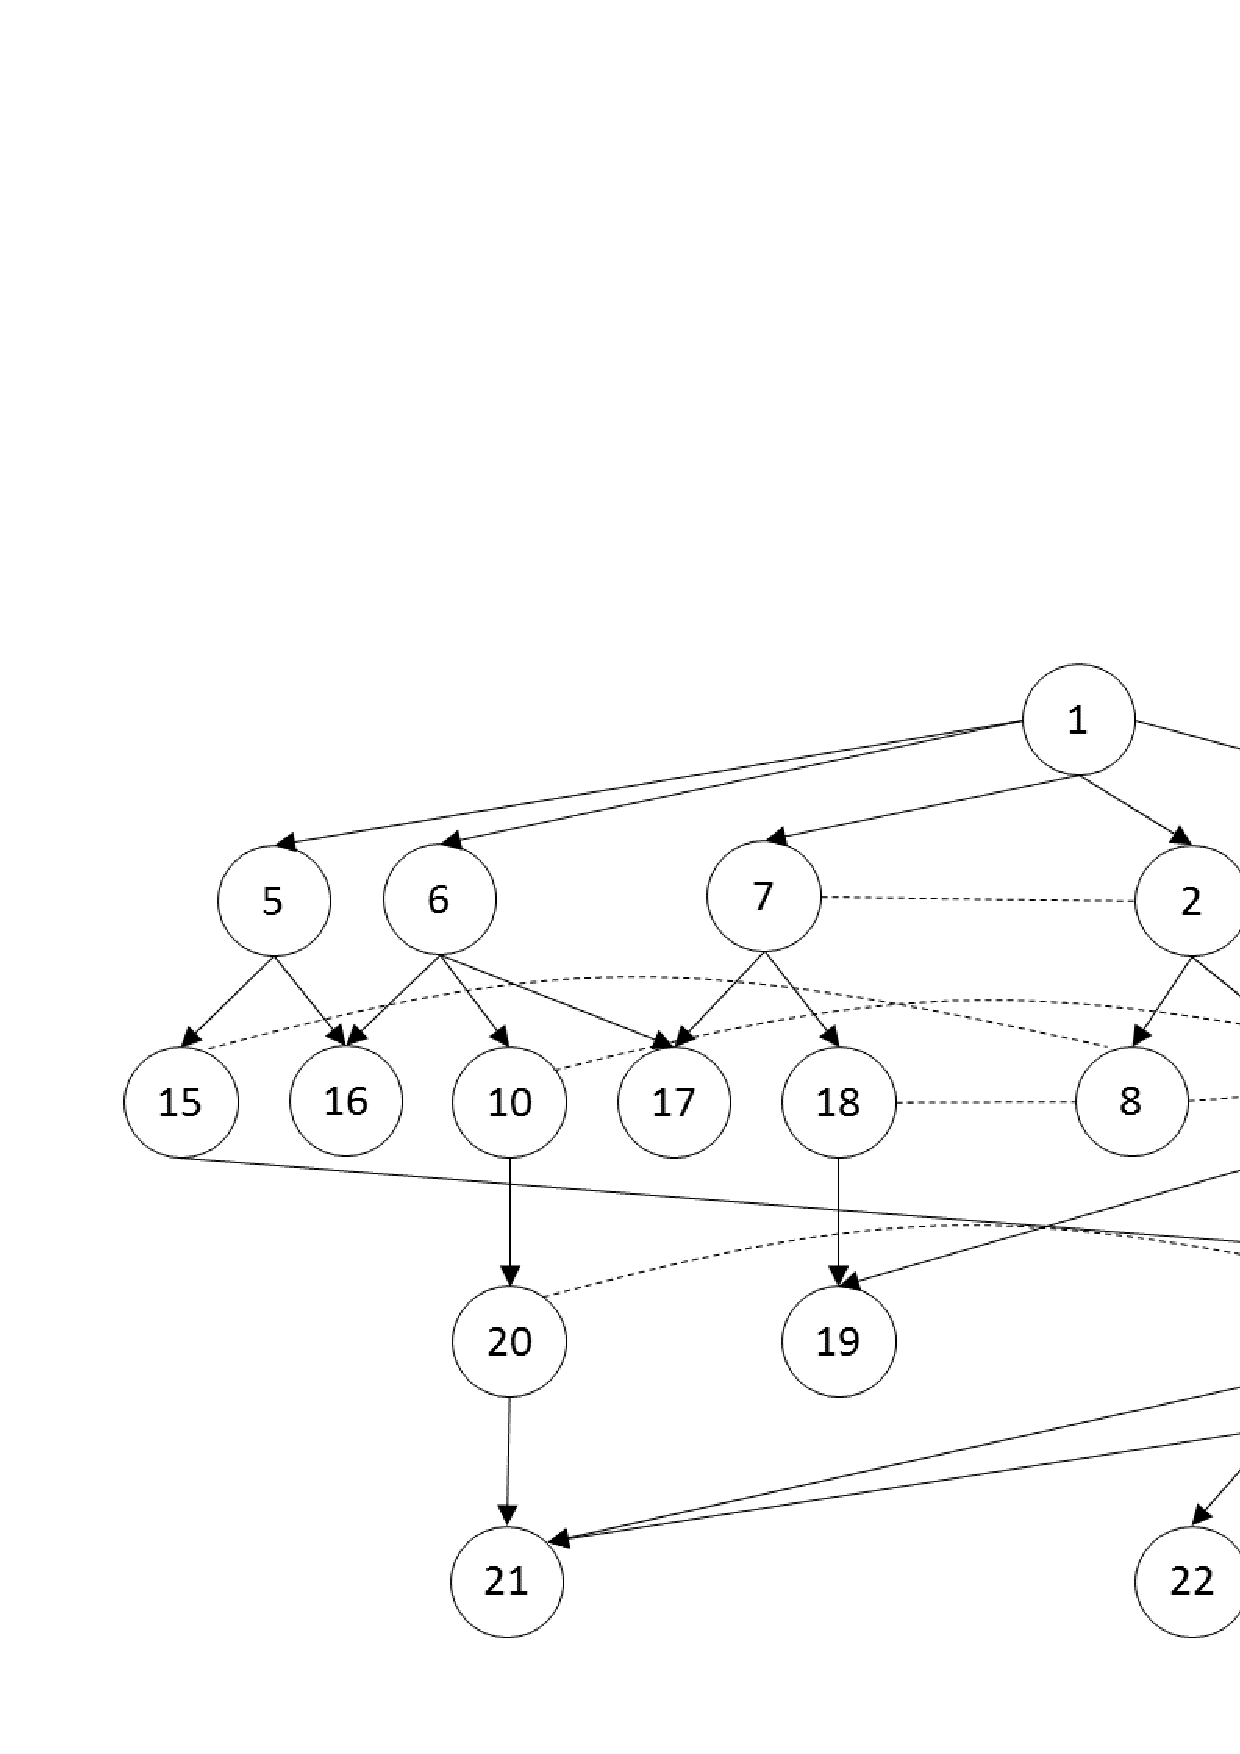
\includegraphics[width=19cm]{images/Slide2.PNG}
\caption{BFS with vertex 1 as source}
\label{fig:exgraph2}
\end{figure}

In Figure \ref{fig:exgraph1}, For vertex 6, vertex 1 is a $parent$, vertex 10 is $cousin$ and vertices 16 and 17 are $ children$. Similarly, For vertex 1, vertex 0 is $parent$, vertex 2 is $cousin$ and vertices 5, 6 and 7 are $children$. 

For source vertex $w$, $parent$ and $cousin$ remain to be an empty set.
For example, in Figure \ref{fig:exgraph1}, vertex 0 has no $parent$ and no $cousin$.
We perform BFS on vertex 0 and obtain information about each vertex's $parent, children, cousins$. Now we re-use these information to perform BFS and compute betweenness centrality for vertex 1 which is shown in Figure \ref{fig:exgraph2}.

Now to compute BFS graph of $u$, $u$ becomes the source and its $sub - tree$ in graph of $v$ remains unchanged.
Vertex 1 and all its reachable vertices in original BFS graph become $sub - tree$ in this BFS graph of $u$ as they remain un-changed in Figure \ref{fig:exgraph2}.

If there are any $cousins$ from $sub - tree$ to outside of $sub - tree$ then they will be $children$ in the new graph. This new relation of $parent$ with their $children$ makes the $children$ to form $extended$ $sub - tree$.
$Cousins$ from $extended$ $sub - tree$ gets changed to their $children$ and thus a new parent child link is formed.
In Figure \ref{fig:exgraph2}, vertex 2 becomes $child$ of vertex 1, because vertex 2 was $cousin$ in Figure \ref{fig:exgraph1} and vertex 1 belongs to $sub - tree$. Also, vertex 10 becomes $child$ of vertex 6, because vertex 10 was $cousin$ in Figure \ref{fig:exgraph1} and vertex 6 belongs to $sub - tree$. This makes vertex 2 and 10 and their reachable vertices which are not included in $sub - tree$ in Figure \ref{fig:exgraph1} to be included to $extended$ $sub - tree$. Thus vertices 8, 9, 10, 20 are included in $extended$ $sub - tree$. Also cousins from $extended$ $sub - tree$ not belonging to $sub - tree$ and $extended$ $sub - tree$ becomes their $children$. For example, vertex 12 becomes $child$ of vertex 9 in Figure \ref{fig:exgraph2} because vertex 12 is not included in any $sub - tree$. 

Hence, we can construct BFS graph of $u$ using BFS graph for $v$.
$\sigma$ values can be easily calculated while making and breaking the links. Then we apply back propagation phase of Brandes' algorithm to calculate Betweenness Centrality. 

The shortcoming of this algorithm is that it takes up a huge amount of space as we need to store graphs for each vertex. Other reason is due to random access nature of memory requirement, improvement in execution time was not achieved. The time complexity remains same as Brandes' algorithm but execution time does not decrease compared to Algorithm \ref{algo:brande}.






